\subsubsection{Schritt 5: Durchf�hren der Tests}\label{sem_eval_step5}
Die Testf�lle aus der Testklasse werden �ber die Annotation @QueryTypeTest ermittelt und sequentiell ausgef�hrt. Als Ergebnis der Testausf�hrung f�r eine ben�tigte Komponente wird ein Objekt des Typs TestResult zur�ckgegeben. Tritt bei der Testausf�hrung eine Exception auf, wird diese im TestResult-Objekt hinterlegt. Im Anschluss wird das TestResult-Objekt direkt zur�ckgegeben, um die Ausf�hrung der �brigen Tests zu verhindern. Wenn ein Test mit positivem Ergebnis durchgef�hrt wird, wird das Attribut passedTests im TestResult-Objekt inkrementiert. Sollten alle Tests erfolgreich durchgef�hrt worden sein, wird das TestResult-Objekt zur�ckgegeben.
\myparagraph{Umgang mit kombinierten angebotenen Komponenten}
Ab dem zweiten Durchlauf werden werden die ben�tigten Komponenten in Schritt 3 aus Kombinationen von Typ-Konvertierungsvarianten mehrere angebotener Interfaces erzeugt. Das f�hrt dazu, dass die Methodenaufrufe auf dem erwarteten Interface an unterschiedliche angebotene Komponenten delegiert werden. Hierbei kann der Fall eintreten, dass mehrere dieser Methoden von der Semantik her auf den gleichen Daten operieren m�ssen, die Aufrufe dieser jedoch an unterschiedliche Komponenten delegiert werden, welche auch auf unterschiedlichen Daten operieren.\\\\
Ein Beispiel hierf�r w�re ein Stack, der durch das erwartete Interface Stack beschrieben. Dieses enth�lt eine push und eine pop Methoden mit der ein Element im Stack hinzugef�gt bzw. entfernt werden kann (siehe \abbref{expected_stack}). Hierbei ist anzunehmen, dass die beiden Methoden auf denselben Daten arbeiten, sodass nach dem Hinzuf�gen eines Elements a (push(a)) und dem darauf folgenden Aufruf der Methode pop() als R�ckgabewert wieder das zuvor hinzugef�gte Element a geliefert wird (siehe \abbref{sd_stack_1}). Wenn die beiden Methoden-Aufrufe jedoch an zwei unterschiedliche Objekte StackA und StackB delegiert werden, die auf unterschiedlichen Daten operieren, dann w�rde dieses Verhalten nicht nachgewiesen werden k�nnen (siehe \abbref{sd_stack_2}).

\begin{figure}[H]
\begin{minipage}[b]{.24\linewidth}
  \centering
  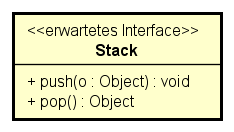
\includegraphics[width=\linewidth]{expected_stack}
  \caption{Erwartetes Interface Stack}
  \label{abb:expected_stack}

\end{minipage}%
\hspace{.04\linewidth}% Abstand zwischen Bilder
\begin{minipage}[b]{.72\linewidth}


  \centering
  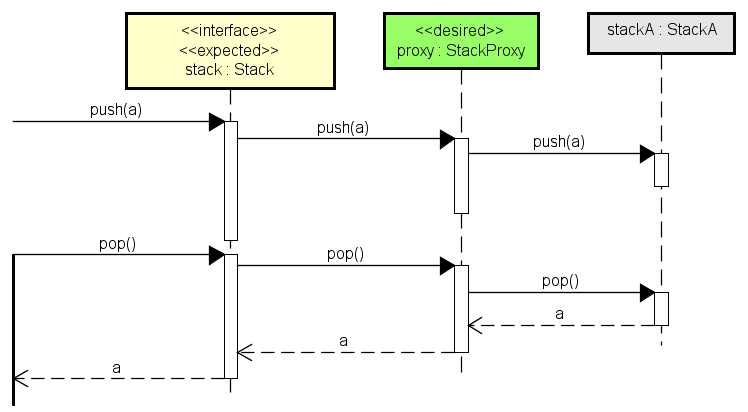
\includegraphics[width=\linewidth]{sd_stack_1}
  \caption{Delegation der Stack-Methoden an genau eine angebotene Komponente}
  \label{abb:sd_stack_1}

\end{minipage}
\end{figure}


%\myBigFigure{expected_stack}{Erwartetes Interface Stack}{expected_stack}
%\myBigFigure{sd_stack_1}{Delegation der Stack-Methoden an genau eine angebotene Komponente}{sd_stack_1}
\myBigFigure{sd_stack_2}{Delegation der Stack-Methoden an unterschiedliche angebotene Komponenten}{sd_stack_2}
\noindent
In einem solchen Fall sollte der Zusammenhang dieser erwarteten Methoden in den Tests spezifiziert werden, sodass diese besonderen semantischen Anforderungen in diesem Schritt evaluiert werden k�nnen. \lstref{LST_StackTest} zeigt ein Beispiel bezogen auf das Szenario aus \abbref{sd_stack_1}.
\begin{lstlisting}[{caption = Testklasse f�r ein erwartetes Interfaces Stack
},{label = LST_StackTest}]
public class StackTest {

  private Stack stack;

  @QueryTypeInstanceSetter
  public void setProvider( Stack stack ) {
    this.stack = stack;
  }

  @QueryTypeTest
  public void pushPop() {
    Object a = new Object();
    stack.push( a );
    Object evalObj = stack.pop();
    assertTrue( a == evalObj );
  }

}
\end{lstlisting}
